% Условная компиляция для самостоятельной работы
\ifdefined\mainfile
    % Если это часть основного файла, не добавляем начало и конец документа
\else
    \documentclass[12pt, a4paper]{report}
    \usepackage{/Users/vladbelousov/Desktop/Semestr_4-FP-NSU/Настройка/library}
    \usepackage[utf8]{inputenc} % Подключение поддержки UTF-8
    \begin{document}
\fi

%%-------------------------------%%

\section{Продолжение теории Гюйгаса-Френеля}

\begin{center}
    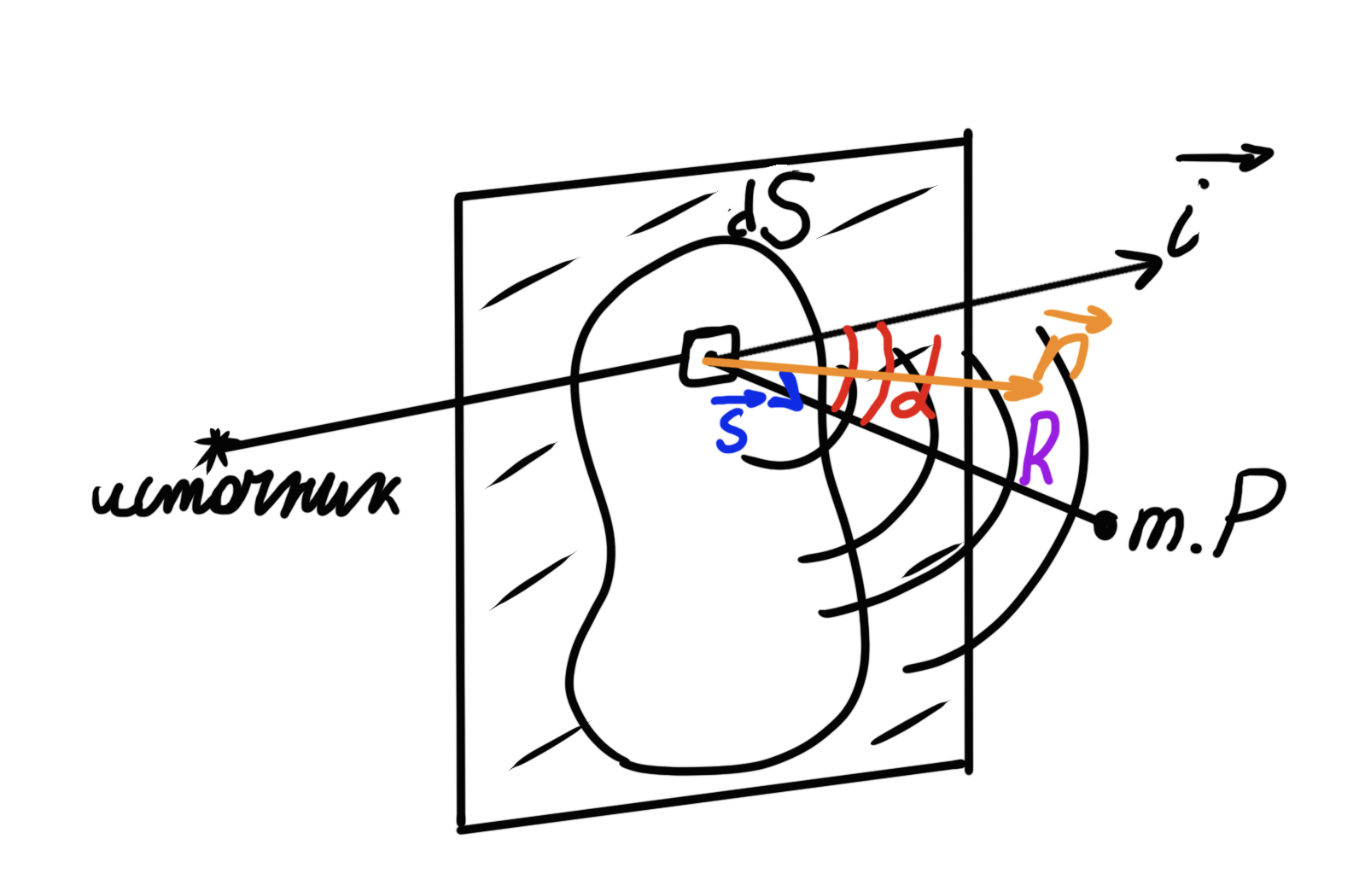
\includegraphics[width=0.5\textwidth]{/Users/vladbelousov/Desktop/Semestr_4-FP-NSU/ЭиО/Лекции_по_дням/image/125.png}
\end{center}
\( \vec{i }  , \vec{s}  \) - единичные вектора, \( \vec{n }  \) - нормаль к поверхности, а  \( \alpha = \widehat{\vec{i},\vec{s}  }  \) 

\[ E_p = \int  \mathbb{K} (\alpha ) E (S ) \frac{e^{ i k R }  }{R } d S_n  \] 

Основные допущения теоремы Гюйгаса-Френеля: 

1) поле в отверстии экрана такое же как и в его отсутствии; 

2) экран абсолютно поглощающий, поле непосредственно за экраном поле равно нулю; 

3) существенна только форма отверстия, несущественна форма его края и материал.

Математическая постановка задачи и нахождение \( \mathbb{K}(\alpha ) \)  - Кирхгоф. 

\[ \Delta E (\vec{r }   ) + k ^2 E (\vec{r } ) = 0  \text{ - скалярное волновое уравнение}  \]

Граничные условия: 

\begin{center}
    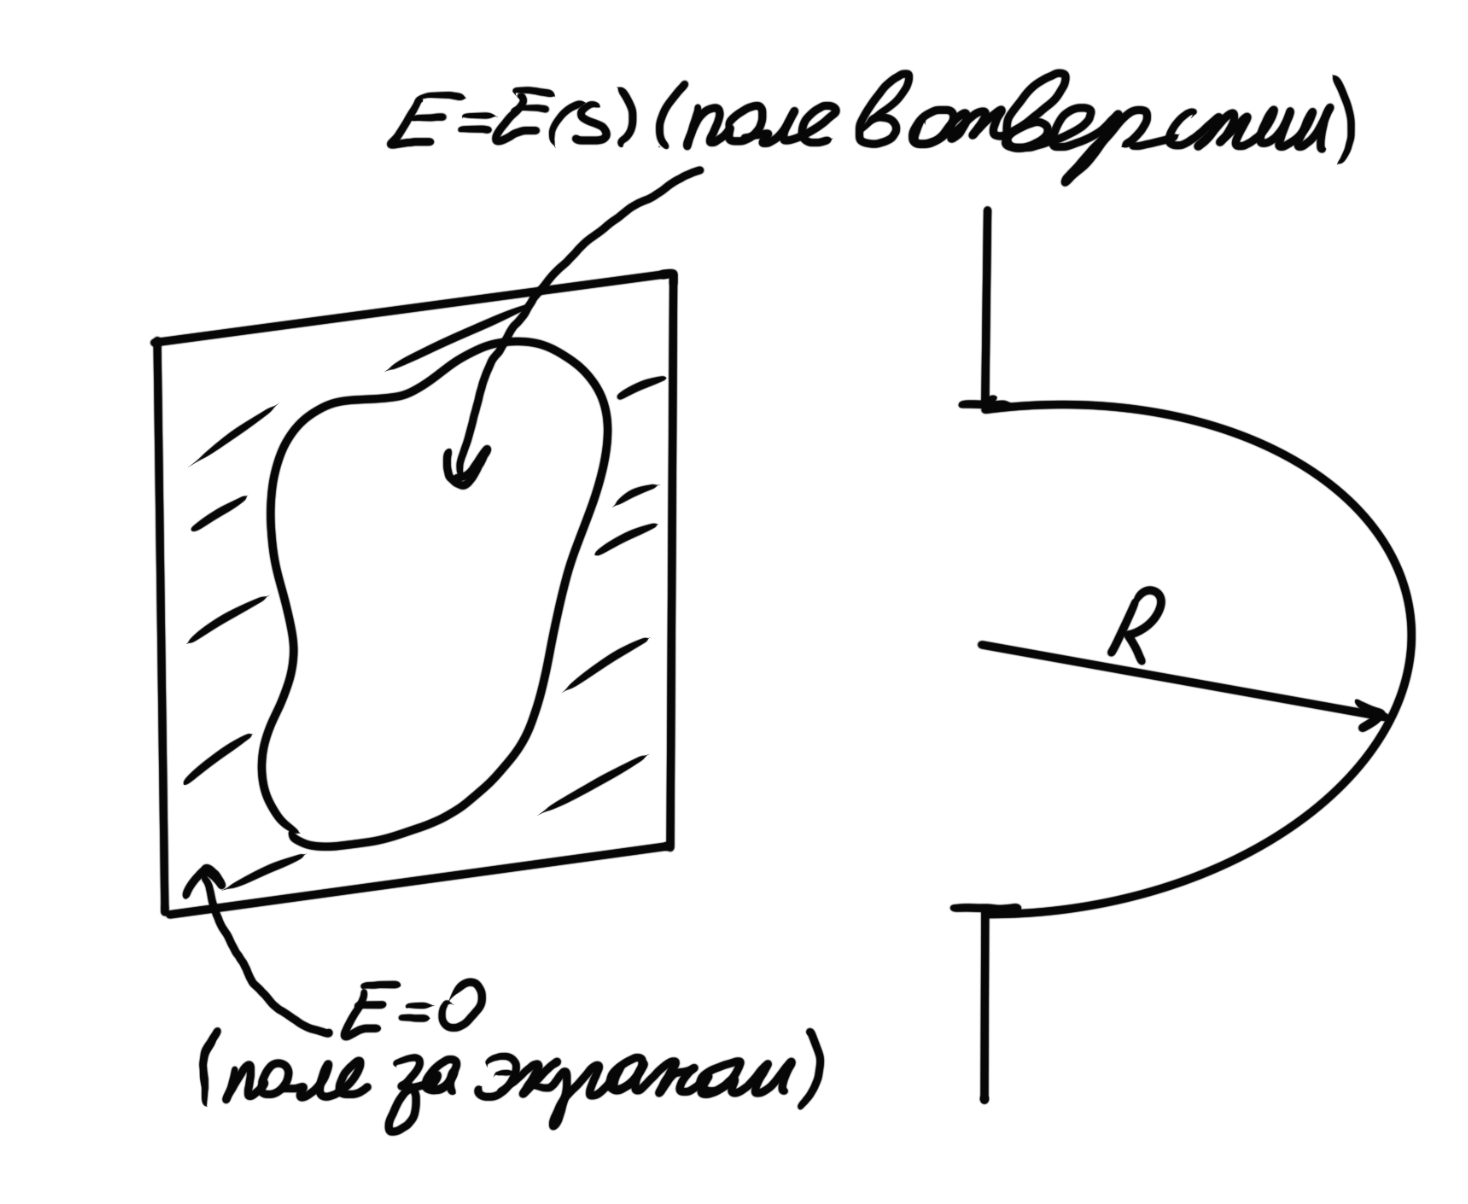
\includegraphics[width=0.5\textwidth]{/Users/vladbelousov/Desktop/Semestr_4-FP-NSU/ЭиО/Лекции_по_дням/image/126.png}
\end{center}
условие излучения (все волны покидают этот объем \( V \) )

\[ E_p = \frac{k}{4 \pi i } \int  d S_n (1 + \cos  \alpha ) \frac{e^{ i k R }        }{ R } E(S )   \] 
\[ \mathbb{K}    (\alpha ) = \frac{k}{4 \pi i } (1 + \cos  \alpha )   \] 
, при \( \alpha \ll 1  \) (параксиальное приближение ) \( \displaystyle  \mathbb{K}     (\alpha ) \approx \frac{k}{2 \pi i}  \) 

\[ \mathbb{K}   = \frac{k}{4 \pi i } \left( \cos ( \widehat{\vec{i } ,\vec{n} }) + \cos (\widehat{\vec{n } , \vec{s} }) \right)  \] 

Вычислим \( \mathbb{K}(\alpha) \) в параксиальном приближении на примере круглого отверстия: 

\begin{center}
    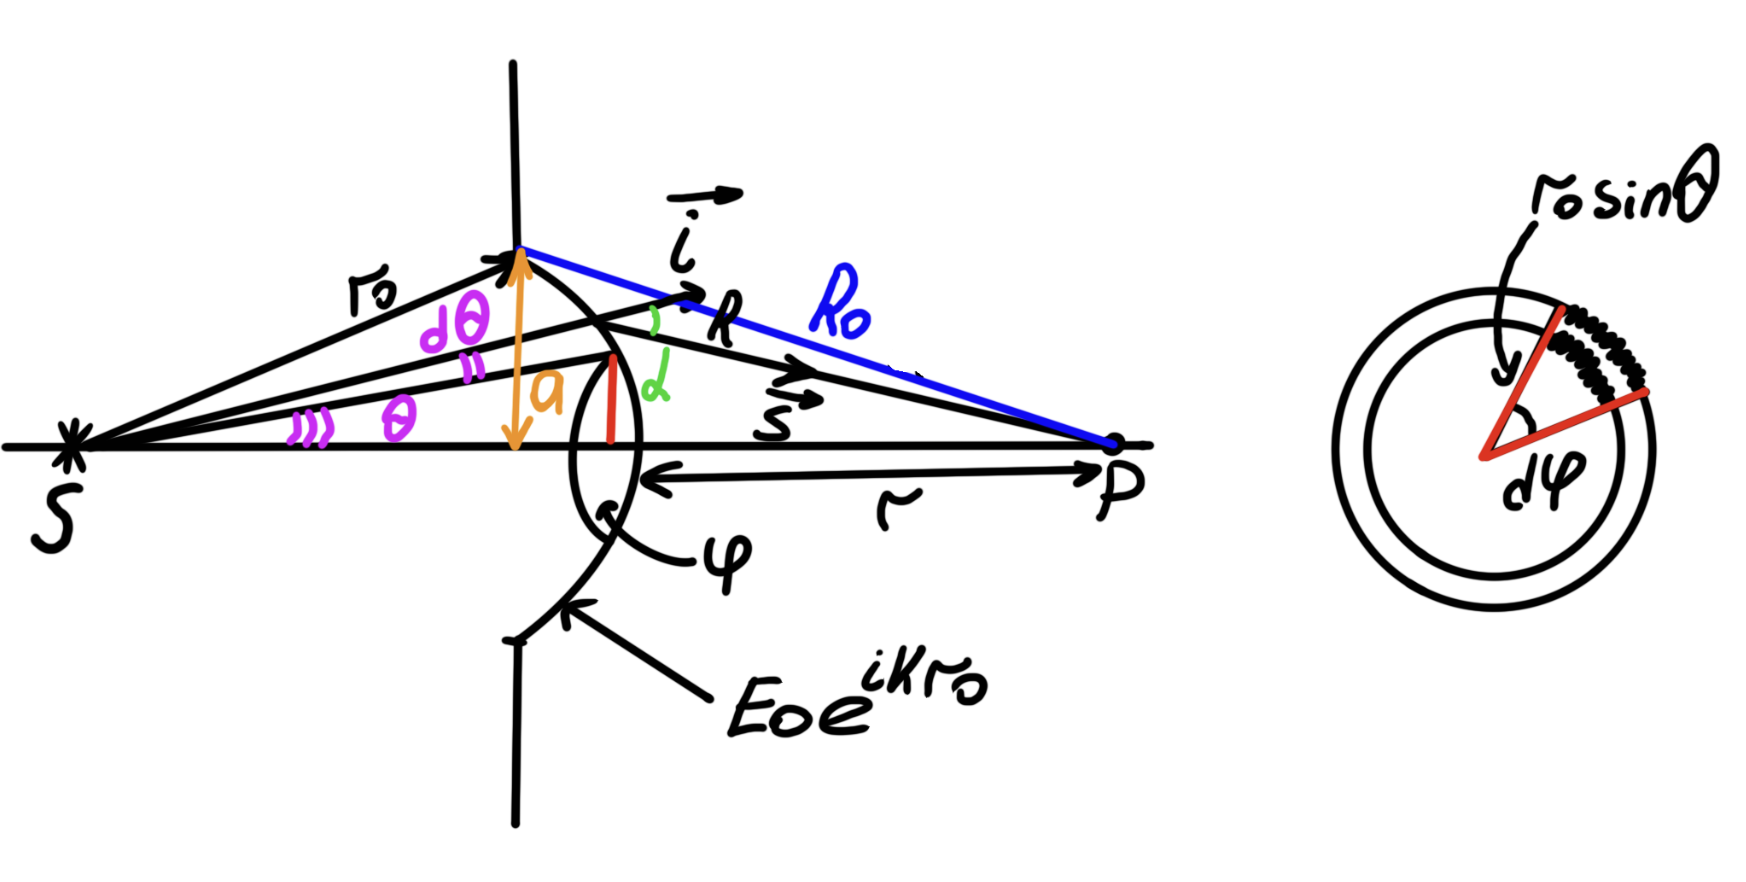
\includegraphics[width=0.7\textwidth]{/Users/vladbelousov/Desktop/Semestr_4-FP-NSU/ЭиО/Лекции_по_дням/image/127.png}
\end{center}

\[ d S_n = d S = r_0 \sin  \theta d \varphi r_0 d \theta \] 

\[ E_p = \iint \mathbb{K}(0 ) E_0 e^{ i k r_0} \frac{e^{i k R } } {R } r_0 ^2 \sin  \theta d \theta d \varphi     \] 

\[ R ^2 = (r_0 +r   ) ^2 + r_0 ^2 - 2 r_0 (r_0 + r  ) \cos  \theta\] 
\[ 2 R d R = 2 r_0 (r_0 + r ) \sin  \theta d \theta \Rightarrow \sin  \theta d \theta = \frac{ R d R }{r_0 (r + r_0)}  \] 

\[ E_p = \mathbb{K} (0 ) E_0 e^{i k r_0} 2 \pi \int \frac{ e^{i k R } }{R } r_0 ^2 \frac{ R dR }{r_0 (r_0 +r)}    \] 
\[ E_p = \mathbb{K} (0 ) \frac{ E_0 e^{ i k r_0 } }{\displaystyle \frac{r_0 + r }{r_0} }  2 \pi \frac{ e^{i k R_0 } - e^{ i k r} }{i k  } = \frac{\mathbb{K} (0 )2 \pi }{k }\underbrace{ \frac{ E_0 e^{ i k (r_0 +r )} }{\displaystyle  \frac{r_0 +r }{r_0} }}_{(*)} \underbrace{\left\{  \frac{e^{ i k (R_0 -r )} -1 }{i} \right\} }_{f(R_0 -r)}  \] 
, где \( (*) \) поле точечного источника в отсутствии экрана \( = E_{P_0}  \) 

\begin{center}
    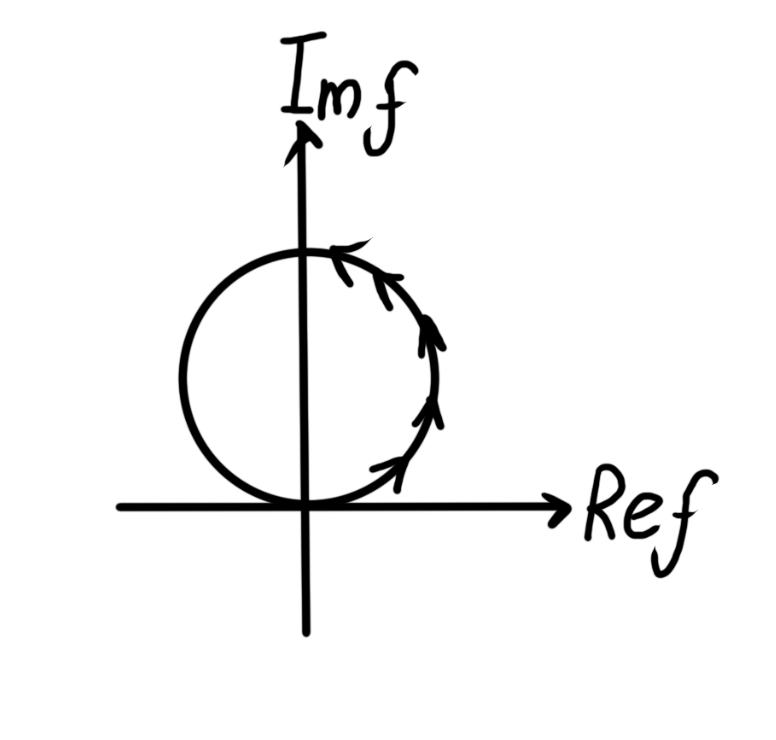
\includegraphics[width=0.3\textwidth]{/Users/vladbelousov/Desktop/Semestr_4-FP-NSU/ЭиО/Лекции_по_дням/image/129-1.png}
\end{center}
,где \( \displaystyle  I = \frac{|E_p| ^2 }{2}  \) 

\[ |f(R_0 - r)| ^2  = (e ^{ i k (R_0 - r)} -1)(e^{ - ik (R_0 - r)} - 1)= 2 -2 \cos (k(R_0 - r)) = 4 \sin ^2 \left( \frac{k (R_0 -r)}{2}  \right)\] 

\begin{center}
    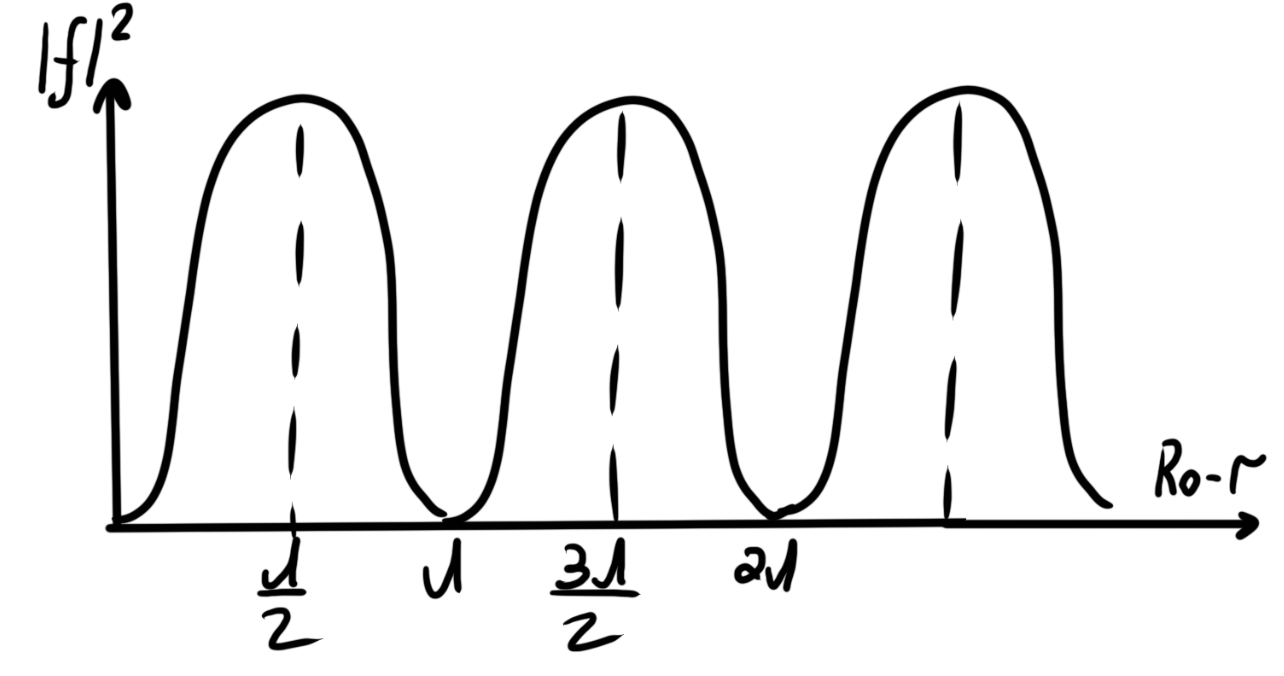
\includegraphics[width=0.5\textwidth]{/Users/vladbelousov/Desktop/Semestr_4-FP-NSU/ЭиО/Лекции_по_дням/image/129.png}
\end{center}

\begin{center}
    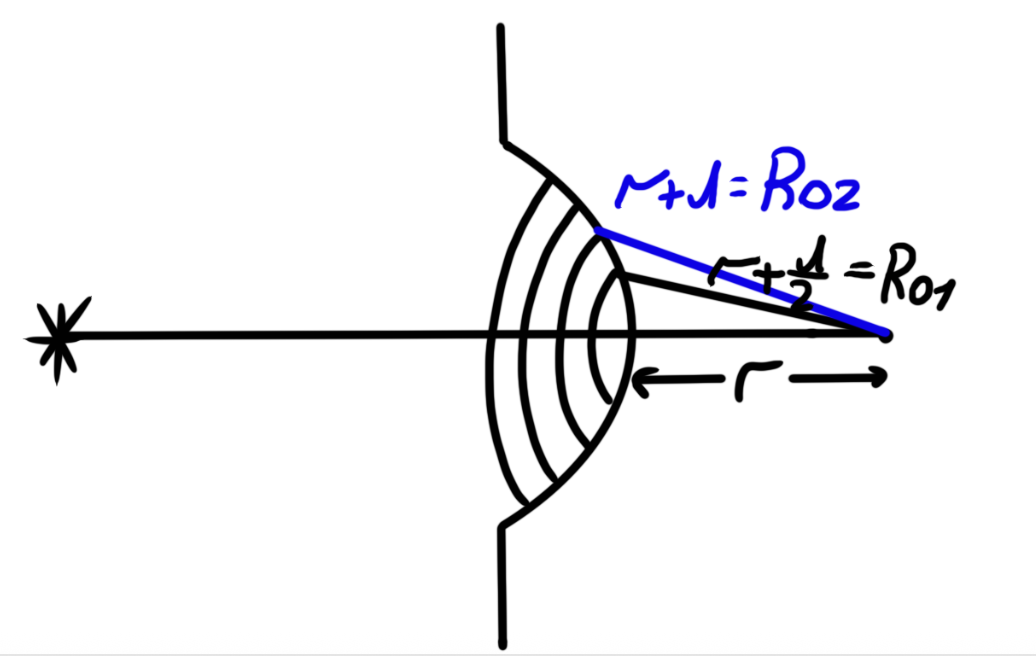
\includegraphics[width=0.5\textwidth]{/Users/vladbelousov/Desktop/Semestr_4-FP-NSU/ЭиО/Лекции_по_дням/image/130.png}
\end{center}

\[ \frac{k (R_{01} - r)}{2} = \frac{\pi}{2 }   \] 
\[ R_{01} -r = \frac{\lambda}{2 }  \] 
\[ R_{0m} - r = m \frac{\lambda}{2}   \] 

Устремим радиус  отверстия к \( \infty  \) и учтем спад \( \mathbb{K} (\alpha) \) с ростом \( \alpha  \Rightarrow\) 
\[ \Rightarrow E_{p_0} = \frac{\mathbb{K} (0 ) 2 \pi }{k } E_{p_ 0} i \Rightarrow \mathbb{K}(0 ) = \frac{k}{2 \pi i } = \frac{1}{i \lambda }      \] 

\[ R_{0 m }  ^2  =\left( r + m \frac{\lambda}{2 }  \right) ^2\overset{(*)}{ = }(r +r_0 ) ^2 + r_0 ^2 - 2 (r_0 + r )r_0 \left( 1 - \frac{\theta ^2 }{2}  \right)  \] 
, где \( (*) \) - из теоремы косинусов.

С учетом, что \( \theta \approx \sin  \theta = \displaystyle \frac{a_m}{r_0}  \): 

\[ r ^2 +r m \lambda + \cancelto{\scriptsize{0\text{(мало)} }}{\left( \frac{m \lambda}{2 }   \right) ^2} = 2 r_0 ^2 + 2 r r_0 + r ^2 - 2 r_0 ^2 - 2 r r_0 + (r_0 +r ) \frac{a_m ^2 }{r_0 ^2 } r_0  \] 

\[ a_m ^2 = \frac{ r_0 r m \lambda }{r_0 + r } = \frac{m \lambda }{\displaystyle  \frac{1}{r_0 }+ \frac{1}{r}  }   \] 
\[ \pi a_{m+1  }  ^2 - \pi a_m ^2 = \frac{\pi \lambda}{\displaystyle \frac{1}{r_0} +\frac{1}{r}  } =\mathrm{ const }\Rightarrow    \] 
\( \Rightarrow \) площадь колец между зонами Френеля - есть постоянная величина.

Если \( r_0 \to  \infty   \), то падает плоская волна \( \Rightarrow a_m = \sqrt{r m \lambda} \) \\

\textbf{Зонные пластинки:   } 

1) Нечетные зоны открыты, четные закрыты:

\begin{center}
    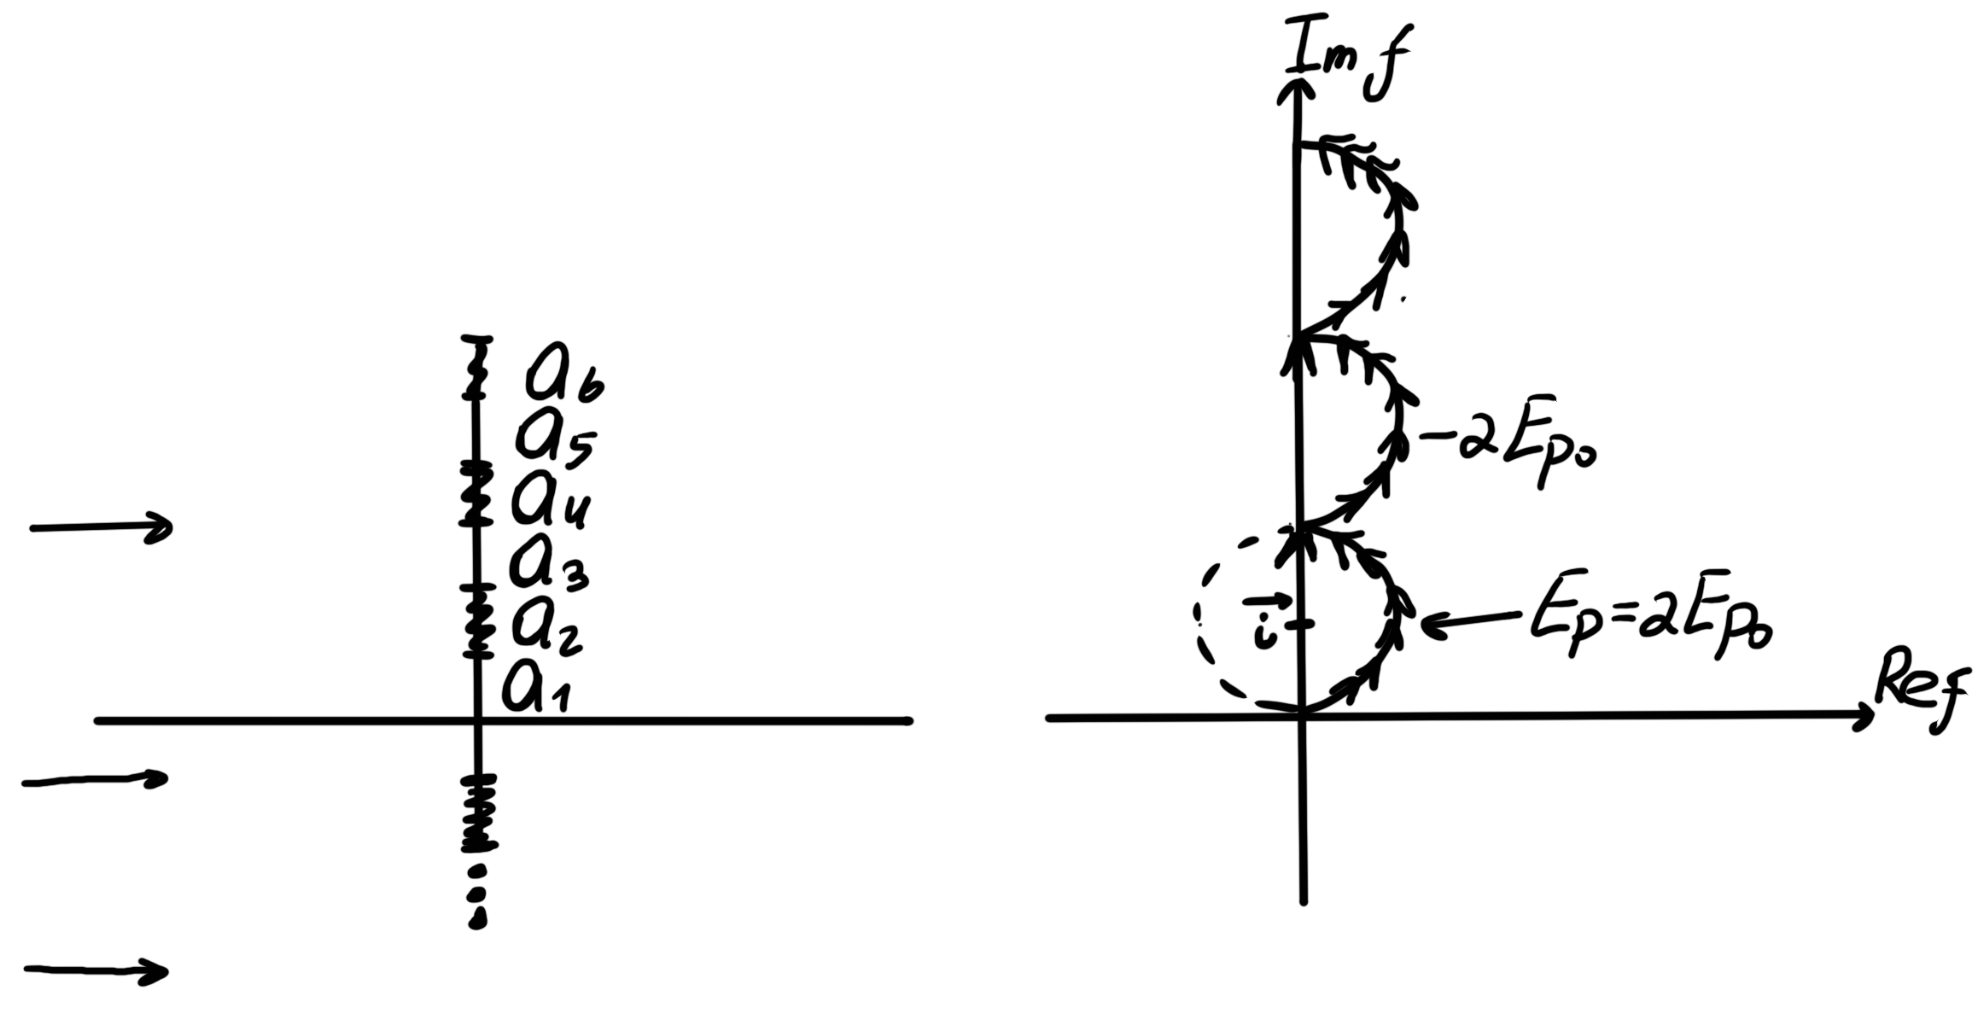
\includegraphics[width=0.7\textwidth]{/Users/vladbelousov/Desktop/Semestr_4-FP-NSU/ЭиО/Лекции_по_дням/image/131.png}
\end{center}


\[ E_p = \frac{k}{2 \pi i } \frac{2\pi}{k }  E_{ p_0} \frac{1}{i }  (e^{i k(R_0 -r)} -1 ) \Rightarrow E_p = E_{p _0 }(1 - e^{i k (R_0 -r)} )    \] 

\( E_{ p _{\Sigma} } = \)\(  E_p \)(от всех нечетных зон)\( =   N \cdot E_{p_0}2 \Rightarrow \) 
\[ \Rightarrow I_{p_{\Sigma} } = \frac{|E_{p_{\Sigma} }| ^2 }{2 } = 4 N ^2 \frac{|E_{p_{0} }| ^2 }{2}  = 4 N ^2 I_0  \] 
, где \( N  \) - число нечетных зон.

2) Нечетные открыты, в четных стоят пластинки, сдвигающие фазу на \( \pi \):

\begin{center}
    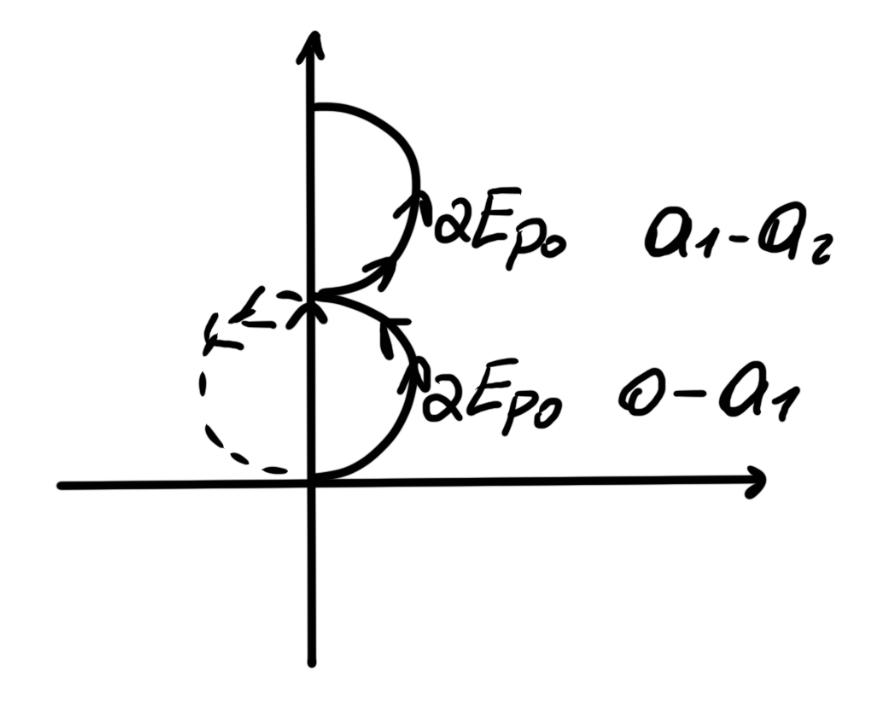
\includegraphics[width=0.3\textwidth]{/Users/vladbelousov/Desktop/Semestr_4-FP-NSU/ЭиО/Лекции_по_дням/image/132.png}
\end{center}

\[ E_{ p_{\Sigma} } =2N E_p \Rightarrow I_{p_{\Sigma} } = 4 N ^2 I_0   \] 
, где \( N \) - число всех зон. 

3) какой то прикол: 

\begin{center}
    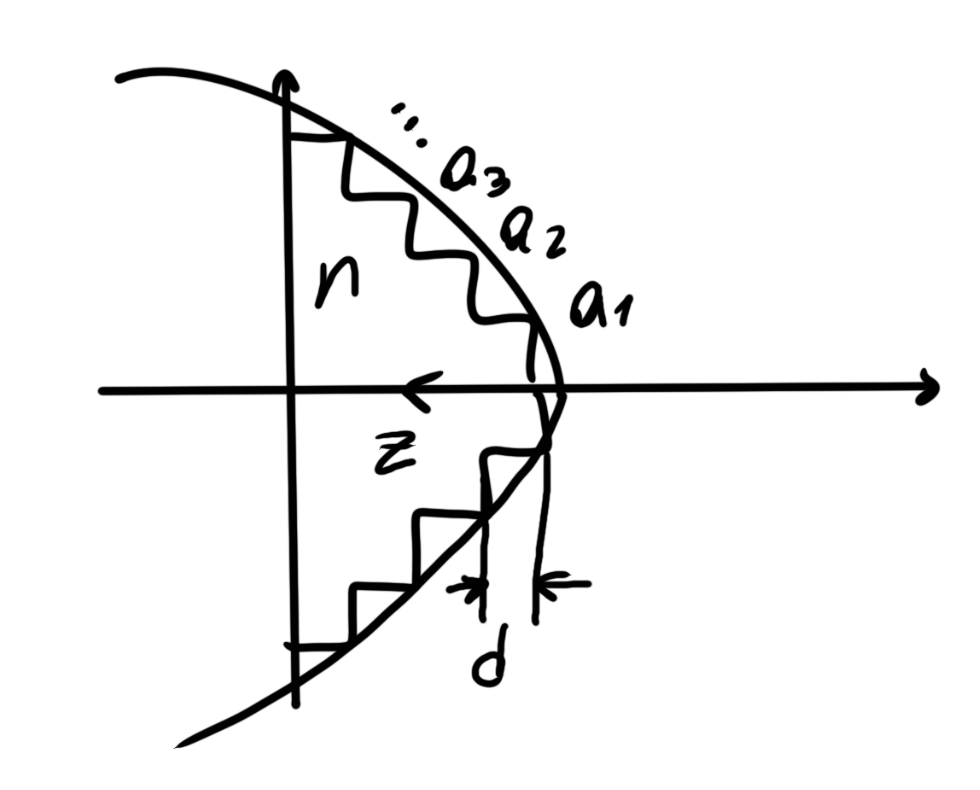
\includegraphics[width=0.4\textwidth]{/Users/vladbelousov/Desktop/Semestr_4-FP-NSU/ЭиО/Лекции_по_дням/image/133.png}
\end{center}

\[ (n-1 ) d = \frac{\lambda}{2 } \Rightarrow \text{сдвиг волн в соседних четных и нечетных зонах }= \pi   \] 

\[ a_m = \sqrt{ m \lambda r} \quad  z_m = (m-1 ) d = (m-1 ) \frac{\lambda}{2 (n-1)}   \] 
\[ z_m = \frac{\lambda}{2(n-1)}\left( \frac{a_m ^2 }{ \lambda r }- 1  \right) \text{ - парабола.}   \] 

\section{Пятно Пуассона и принцип Бабине }

\begin{center}
    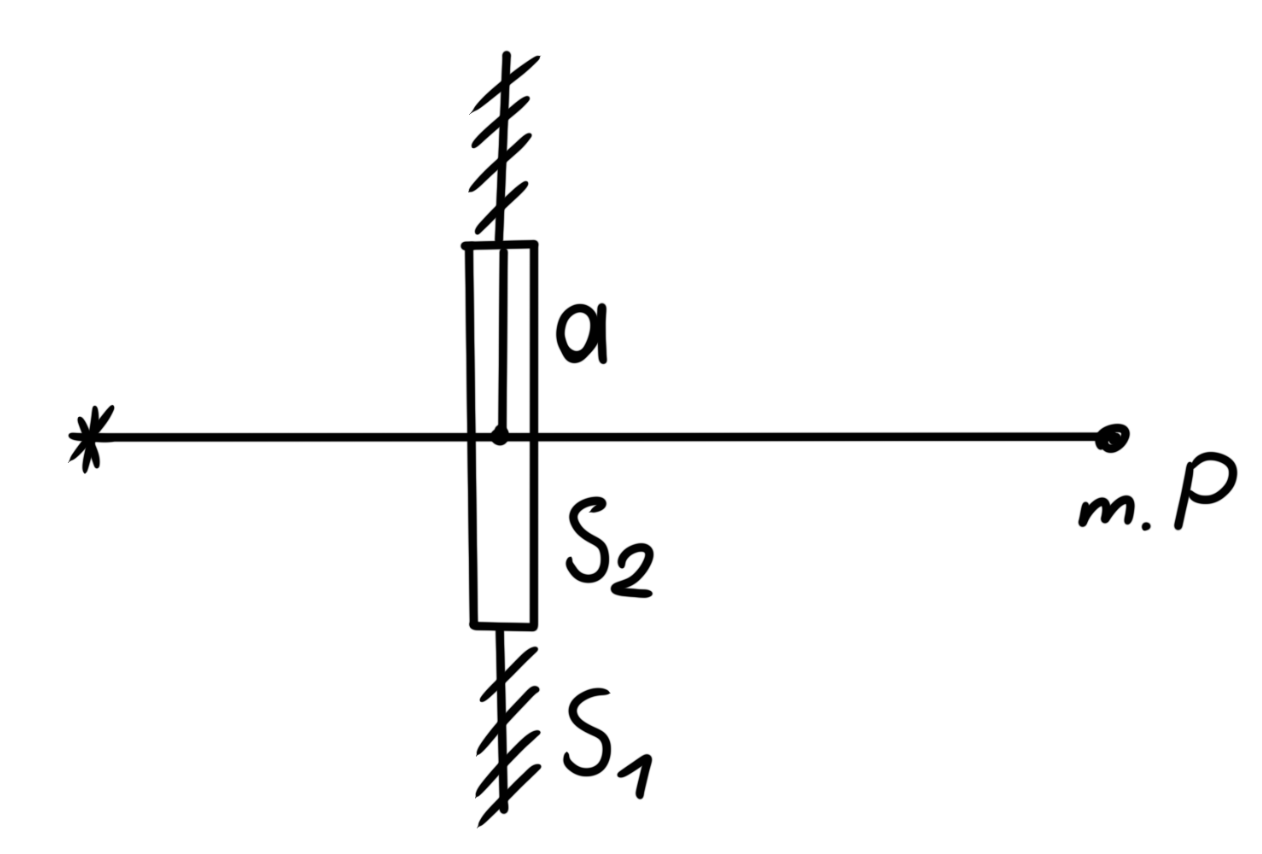
\includegraphics[width=0.5\textwidth]{/Users/vladbelousov/Desktop/Semestr_4-FP-NSU/ЭиО/Лекции_по_дням/image/134.png}
\end{center}

\[ E_p = \frac{k}{2 \pi i } \int_{S_1} E(S) \frac{e^{i kR } }{R} d S_n = \int_{(*)}- \int_{S_2}   \] 
, где \( (*) \) в отсутствии отверстия. И \( \displaystyle \int_{(*)} = E_{p _0}   \), \( \displaystyle \int_{S_2} = E_{p _0} (1- e^{i k (R_0 -r)} )  \) 

\[ \int_{a }^{\infty  }= \int_{0 }^{\infty  }- \int_{0 }^{a} = E_{p_0} e^{ i k (R_0 -r)} \Rightarrow I_p = \frac{|E_{p_0} | ^2 }{2} = I_{p_0}       \] 
%%-------------------------------%%

% Закрытие документа, если файл компилируется отдельно
\ifdefined\mainfile
    % Если это основной файл, не нужно заканчивать документ
\else
    \end{document}
\fi